
\setcounter{chapter}{1}
\chapter{Requirements Analysis and Specification}
\minitoc %insert la minitoc
\graphicspath{{Chapter2/figures/}}

%\DoPToC

%==============================================================================
\pagestyle{fancy}
\fancyhf{}
\fancyhead[R]{\bfseries\rightmark}
\fancyfoot[R]{\thepage}
\renewcommand{\headrulewidth}{0.5pt}
\renewcommand{\footrulewidth}{0pt}
\renewcommand{\chaptermark}[1]{\markboth{\MakeUppercase{\chaptername~\thechapter. #1 }}{}}
\renewcommand{\sectionmark}[1]{\markright{\thechapter.\thesection~ #1}}

\begin{spacing}{1.2}
%==============================================================================
\section*{Introduction}
In this chapter, we will begin our project with a study of the existing checkout developers API's on the market. We will then start the requirements analysis. This will help us identify the different actors that will interact with our system, as well as the features required in our project.
\section{Study of the Existing Market}
In the world of e-commerce, a variety of payments methods exist.  Most of these methods are credit card related and offer the possibility of paying using the card number and the three-digit code.

In our case, Flouci offer payments through QR codes scans. Although the payment steps on the user side are different, the developer's API should offer similar functionalities.


Below is a list of world leader online payments API's:
\begin{itemize}
  \item \textbf{Stripe:}

 The Stripe \cite{stripe} API is organized around REST. The API has predictable resource-oriented URLs, accepts form-encoded request bodies, returns JSON-encoded responses, and uses standard HTTP response codes, authentication, and verbs.

You can use the Stripe API in test mode, which does not affect your live data or interact with the banking networks. The API key you use to authenticate the request determines whether the request is live mode or test mode.

The figure \ref{fig:stripe} shows the code behind Stripe integration.
\begin{figure}[H]\centering
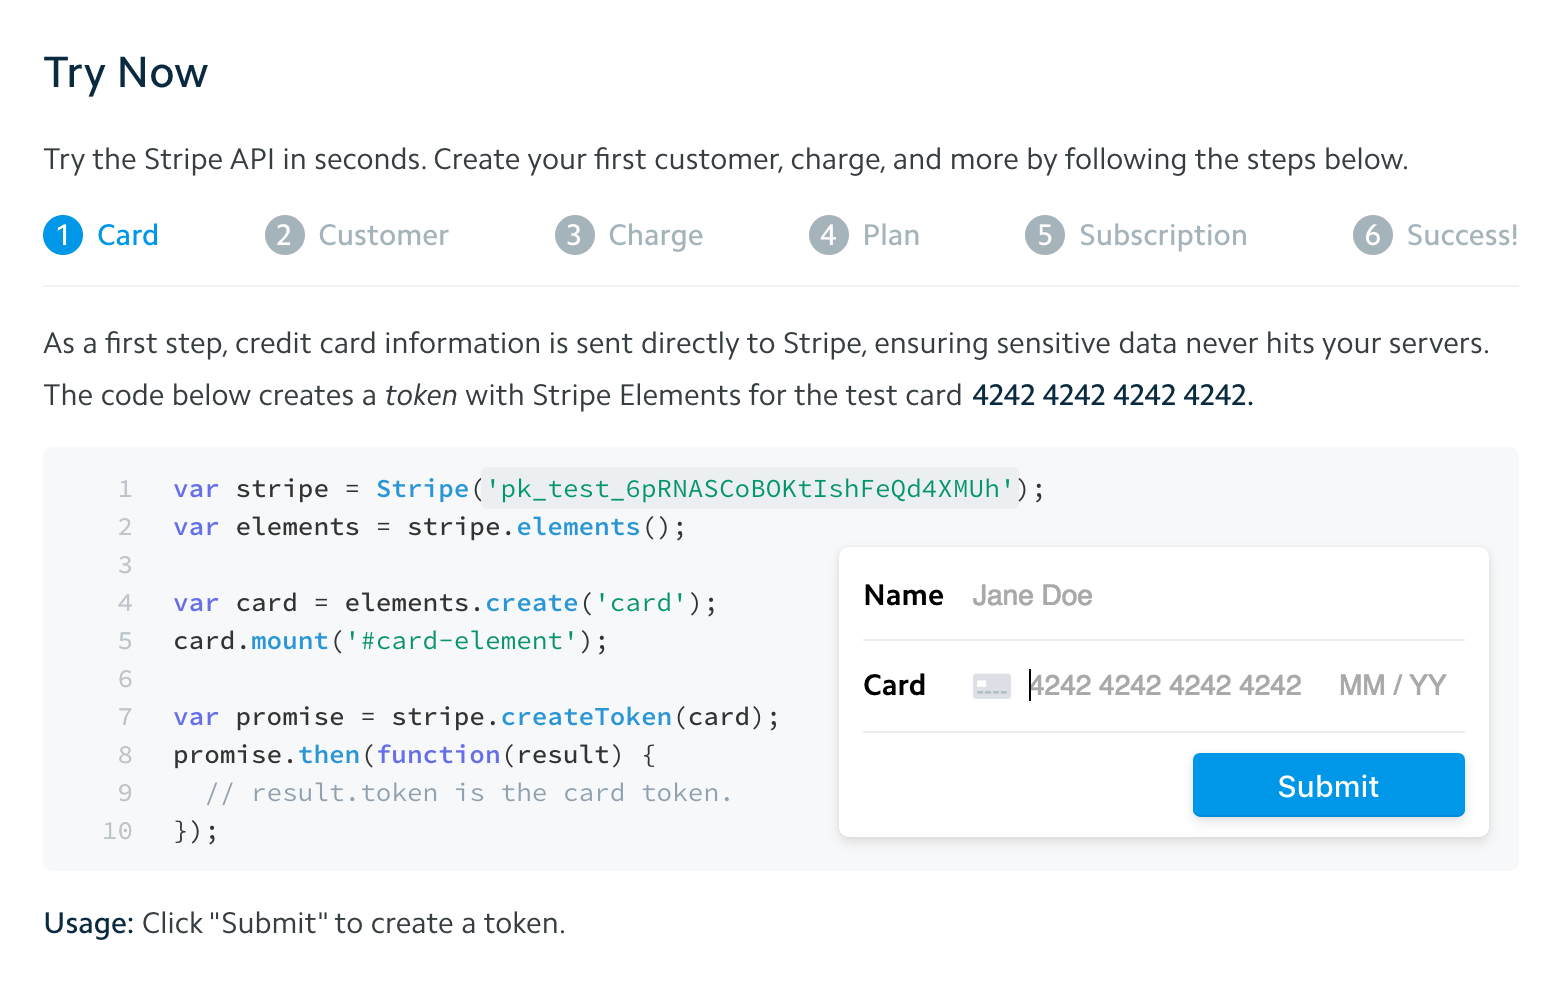
\includegraphics[scale=0.3]{stripe.png}
\caption{Stripe API}
\label{fig:stripe}
\end{figure}

  \item \textbf{PayPal:}

  The PayPal \cite{paypal} APIs are HTTP-based RESTful APIs that use OAuth 2.0 for authorization. API request and response bodies are formatted in JSON.

The figure \ref{fig:paypal} shows the developer's API of PayPal.
\begin{figure}[!ht]\centering
\includegraphics[width=\textwidth,height=6cm]{PayPal.png}
\caption{PayPal API}
\label{fig:paypal}
\end{figure}

\item \textbf{Twint:}

Twint \cite{twint} is the closest implementation to Flouci as it offers payments through QR code scans.

The plugin allows QR code generation on the web page, it also creates a code for each transaction that serves to confirm payments.
The figure \ref{fig:twint} shows the Twint payment interface.

\begin{figure}[H]\centering
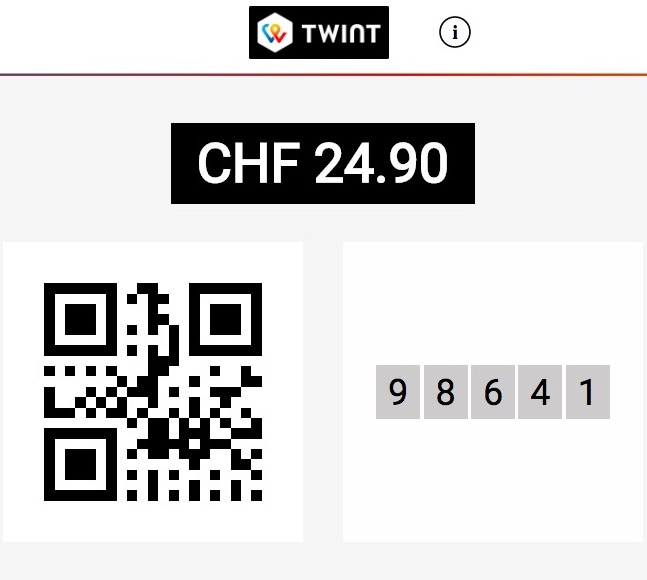
\includegraphics[scale=0.3]{twint.jpg}
\caption{Twint Pop-up}
\label{fig:twint}
\end{figure}
  \end{itemize}



\section{Requirements Specification}
A good in-depth requirements specification is the key to a solid foundation of any project.
The motivation behind this section is to take a global look at the project and be able to understand all the requirements needed to achieve our goals.
\subsection{Actors Identification}
Actors are any entity that plays a role in our system. They can be users or systems that interact with our system. We were able to identify the external and internal actors of our platform.
\newline
Among the internal actors we find:
\begin{itemize}
  \item \textbf{Anonymous Developer:} She can navigate on all the public pages of the site which are
accessible without authentication including the documentation part. Also, she can register a developer account.
  \item \textbf{Registered Developer:} She can manage her account, create and manage app's and integrate them on e-commerce websites.
  \item \textbf{Flouci User:}  She can use the checkout API to pay online merchants.
\end{itemize}
The external actors who are necessary for our platform are:
\begin{itemize}
  \item \textbf{Wallets API:} Is needed to activate any app. The app should be linked to a Flouci wallet.
  \item \textbf{Payments API:} Is needed for online payments.
\end{itemize}
\subsection{Functional Requirements}
In this section, we will understand the functional requirements of our project by studying the global use case of our system.
	\newline In the Figure \ref{fig:usecasediagram}, we showcase the \textbf{general use case diagram} and then with the Table \ref{tab:usecasediagram} we will explain more in-depth the different use cases.

\begin{figure}[H]\centering
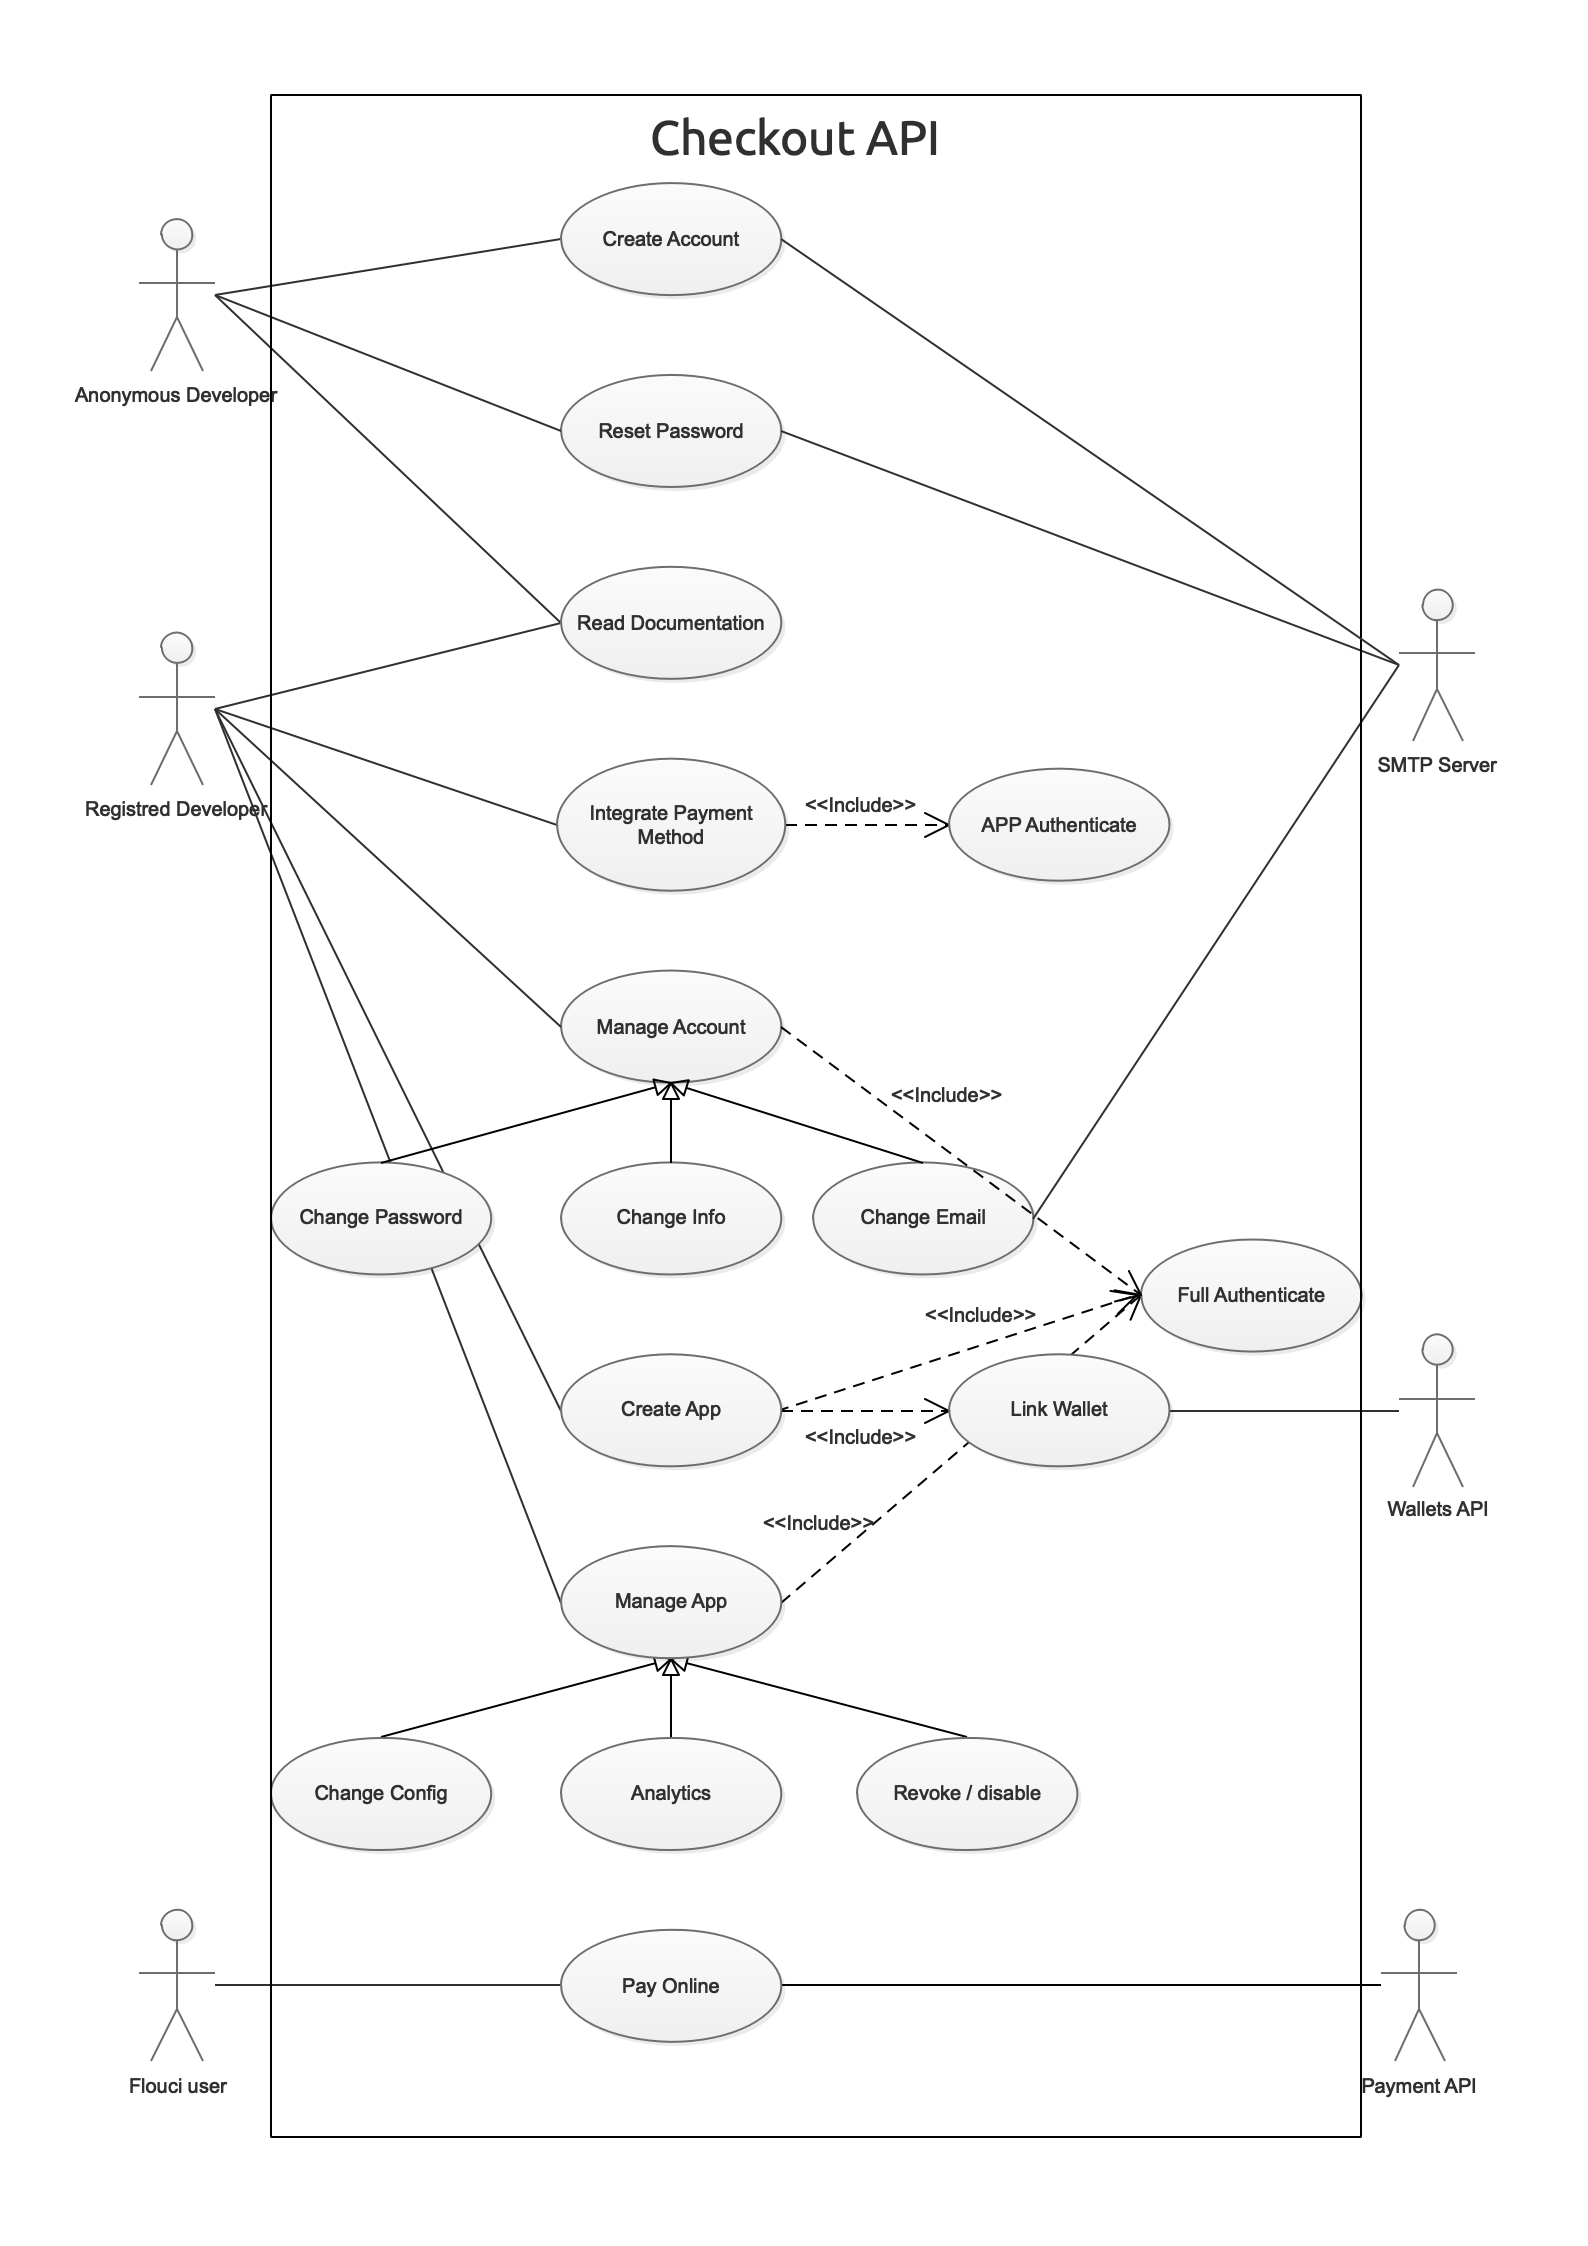
\includegraphics[width=\textwidth,height=\textheight,keepaspectratio]{GeneralUseCase.png}
\caption{General Use Case Diagram}
\label{fig:usecasediagram}
\end{figure}

\begin{table}[!h]
	\centering
	\caption{Use case description table}
	\footnotesize
	\begin{tabularx}
	{\linewidth}{|>{\centering{}\vspace*{\fill}}X|>{\centering{}\vspace*{\fill}}X|>{\vspace*{\fill}}X<{\centering{}}|}
			\hline
			 \bfseries Internal actor & \bfseries Use case &\bfseries External actor \\
			\hline
			\multirow{3}{*}{Anonymous Developer}			&	Create Account: Any person with an email account can register for a Flouci developer account. 	&	SMTP Server			\\
			\cline{2-3}
				& Reset Password: In case a registered user forgets his password, he can reset it using his email address. 		&		SMTP Server		\\
				\cline{2-3}
					&	Read Documentation: Any person with access to the developer's platform can access the documentation.	&				\\
			\hline
			\multirow{5}{*}{Registered Developer}					&	Read Documentation: The developer can access the documentation 	&				\\
			\cline{2-3}
			&	Integrate Payment Method: Any active app could be integrated into a commerce website and the integration only requires the public and private app tokens (App Authentication).	&				\\
			\cline{2-3}
					&	Manage Account:    The developer can change manage her account by changing her password, email or her basic info.	&		SMTP Server	\\
					\cline{2-3}
					&	Create App: An Authenticated developer can create an app and link it to a wallet with OTP verification through the Wallets API.	&			Wallets API	\\
					\cline{2-3}
					&	Manage App:	 An Authenticated  developer can check the analytics of her apps as well as tweak any app settings. &				\\

			\hline
			Flouci User	& Pay Online : With the "pay with Flouci" button on e-commerce websites, the Flouci user can quickly pay online merchants.  	&	Payment API	\\

			\hline
	\end{tabularx}
	\label{tab:usecasediagram}
\end{table}


\subsection{Non-Functional Requirements}
\subsubsection{Security}
When it comes to payment solutions, security is the number one requirement to keep in mind.
Our solution implements many layers of security including:
\begin{itemize}
	\item \textbf{Secure connection:} Since we will be handling payments data each connection should be secure .
	\item \textbf{Authentication / Authorization :}  A clear protocol should be set to handle different access types to our platform.
    \end{itemize}
\subsubsection{Documentation}
An API is only usable with proper documentation. In order to get developers to implement our solutions, we should have easy and understandable documentation. The documentation is accessible in our platform.\subsubsection{Logging}
Our solution is using "logstash" to forward logs to our ELK \cite{ELK} stack. Different log levels are used and we have implemented many metrics and dashboards on our kibana.
The figure below \ref{fig:kibana} shows the logging dashboard of Kibana.
\begin{figure}[H]\centering
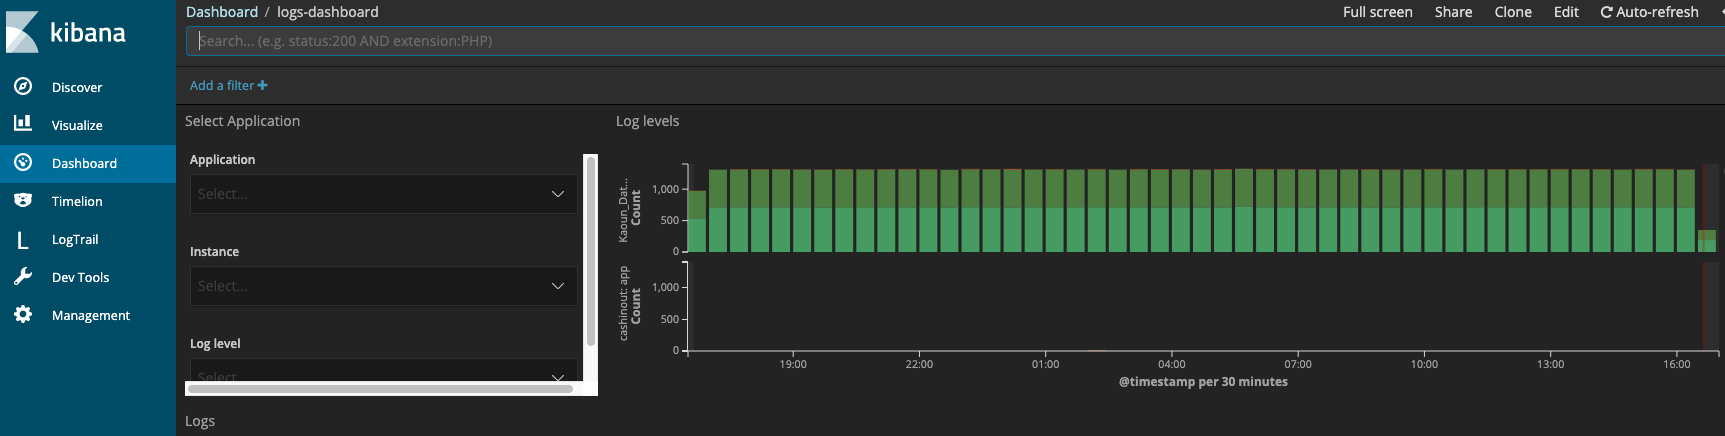
\includegraphics[scale=0.3]{ELK.png}
\caption{Kibana Dashboard}
\label{fig:kibana}
\end{figure}

\subsubsection{Integrability}
Flouci online payment method can be easily integrated into any e-commerce website. It only requires an HTML form in the front end and an API call to accept payments on the backend.

\subsubsection{Extensibility}
Our payment method should allow extensibility and add more payment method other than the QR code scans.
\subsubsection{Legal}
On the legal side, we must be entirely compliant with Tunisian laws and only enable appropriate users to accept payments.
This is achieved on the app creation level, at the stage of linking the wallet.
\subsubsection{Privacy}
Flouci users' privacy should be held to the highest standards. Payment history and activities should be seen only by the persons with the right permissions.
\subsubsection{Ergonomics}
To guarantee a good control of our project and to simplify the interaction with the final users, we support our analysis of functional needs with mock-ups that model the different interfaces of our final product. These models are made by the "Adobe XD" tool and they are compliant with the overall Kaoun prouduct user experience.

\section{Tools}
In the section, we will present the set of tools that make it possible to follow the development disciplines mentioned above. The tools also help the automation of the processes.
\subsection{AdobeXD}
"Adobe XD" \cite{AdobeXD} is a vector-based tool developed and published by Adobe Inc for designing and prototyping user experience for web and mobile apps.
\subsection{Bitbucket}
"Bitbucket" \cite{Bitbucket} is a web-based version control repository hosting service owned by Atlassian, for source code and development projects that use Git revision control systems.
\subsection{GitKraken Glo Boards}
"GitKraken Glo Boards" is a software that manage boards and tickets. In our case the Kanban board is created and managed on GitKraken.
\subsection{Docker}
"Docker" \cite{Docker} is a tool designed to make it easier to create, deploy, and run applications by using containers. Containers allow a developer to package up an application with all of the parts it needs, such as libraries and other dependencies, and ship it all out as one package. By doing so, thanks to the container, the developer can rest assured that the application will run on any other machine regardless of any customized settings that machine might have that could differ from the machine used for writing and testing the code.
\subsection{Docker Swarm}
As a platform, Docker has revolutionized the manner software was packaged. "Docker Swarm" \cite{Dockerswarm} or simply Swarm is an open-source container orchestration platform and is the native clustering engine for and by Docker. Any software, services, or tools that run with Docker containers run equally well in Swarm. Also, Swarm utilizes the same command line from Docker.

Swarm turns a pool of Docker hosts into a virtual, single host. Swarm is especially useful for people who are trying to get comfortable with an orchestrated environment or who need to adhere to a simple deployment technique but also have more just one cloud environment or one particular platform to run this on.
\subsection{Jenkins}
In order to have our CI/CD environment, we used "Jenkins" \cite{Jenkins} which is an open source automation server that helps you to automate the non-human part of the software development process.

"Jenkins" is a stand-alone open source automation server that can be used to automate all kinds of tasks related to software creation, testing, delivery or deployment.
\subsection{SonarQube}
"SonarQube" \cite{SonarQube} (formerly Sonar) is an open-source platform developed by SonarSource for continuous inspection of code quality to perform automatic reviews with static analysis of code to detect bugs, code smells, and security vulnerabilities on 20+ programming languages.

"SonarQube" offers reports on duplicated code, coding standards, unit tests, code coverage, code complexity, comments, bugs, and security vulnerabilities.
\section*{Conclusion}
In this chapter, we reviewed the different aspects of our project. We went through a detailed analysis of function and non -functional requirements in order to comprehend the project boundaries.
Finally, we presented the key tools we will be using in our project development life cycle.

After this, we are able to launch our project development cycles. The first sprint will focus on setting up the right development disciplines and practices to follow in our project.

%==============================================================================
\end{spacing}
